\documentclass[crop,class=article]{standalone}
%----------------------------Preamble-------------------------------%
\usepackage{amssymb}        % For \mathbb{C}.
\usepackage{tikz}           % Drawing/graphing tools.
\usetikzlibrary{
    arrows.meta,            % Latex and Stealth arrows.
    decorations.markings,   % Adding arrows in the middle of a line.
}
%--------------------------Main Document----------------------------%
\begin{document}
    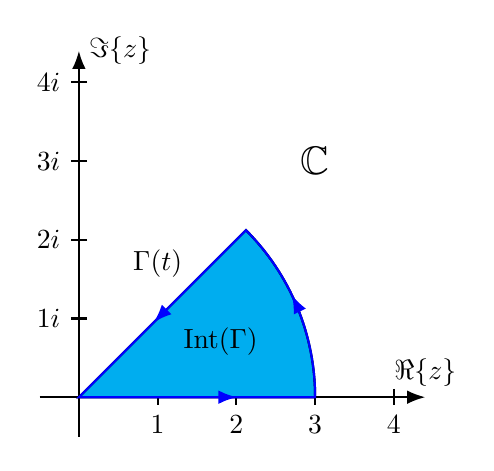
\begin{tikzpicture}[
        >=Latex,
        thick,
        ->-/.style={%
            decoration={%
                markings,
                mark=at position 0.24 with \arrow{>},
                mark=at position .52 with \arrow{>},
                mark=at position .84 with \arrow{>}
            },
            postaction={decorate}
        }
    ]
        \draw[>=Latex, ->] (-0.5, 0) -- (4.4, 0) node[above] {$\Re\{z\}$};
        \draw[>=Latex, ->] (0, -0.5) -- (0, 4.4) node[right] {$\Im\{z\}$};
        \foreach\n in {1,2,3,4}{%
            \draw (\n,3pt) -- (\n,-3pt) node [below] {$\n$};
            \draw (3pt,\n) -- (-3pt,\n) node [left] {$\n{i}$};
        }
        \draw[fill=cyan] (0, 0) to (3, 0) arc(0:45:3) to cycle;
        \draw[blue, ->-] (0, 0) to (3, 0) arc(0:45:3) to cycle;
        \node at (3, 3) {\Large{$\mathbb{C}$}};
        \node at (1, 1.7) {\normalsize{$\Gamma(t)$}};
        \node at (1.8, 0.7) {\normalsize{$\textrm{Int}(\Gamma)$}};
    \end{tikzpicture}
\end{document}